\section{MPC results}
\label{sec:MPC_results}
MPC offers a structure for designing a controller that should be able to stabilize the plant. Nevertheless, there is a multitude of different architectures which may provide different properties. In combination with this, some weights have to be tuned for the controller to prioritize the objectives we want to follow. 

\noindent
Multiple criteria should be upheld.
\begin{itemize}
    \item $F_{st}$ and $F_{O_2}$ should be stabilized and should reject disturbances.
    \item Non-zero mean disturbances should be rejected completely.
    \item The controller should be verifiable through the use of a simulator. 
    \item The ratio between $F_{aI}$ and $F_{aII}$ should only be able to deviate form the pre-determined reference ratio temporarily
    \item In the case where there are hard safety-constraints, the controller should try to uphold these. 
    \item The controller should be well-behaved, even if the inputs have saturation limits or limits to the rate of change. 
\end{itemize}

\noindent 
Normally, an MPC differs somewhat from an LQR in that it can express a cost for the change in variables. The LQR usually has to use high-pass filters to achieve a similar effect. Fortunately, a low-pass filter on the input is already required to control the plant, since both MPCs and simulators are bad at handling feed-through terms through the plant and controller. As a result, the low-pass filter can be used to make a high-pass filter:

\begin{align}
   1 - \frac{1}{\tau_{\text{low pass}} s +1} = \frac{\tau_{\text{low pass}}s}{\tau_{\text{low pass}}s +1} = h_{\text{high pass}}(s)
\end{align}

\noindent
Matlab already has a function $\text{lqry}$, which returns the gain $K_{lqr}$. $K_{lqr}$  optimizes the Ricatti equation if an output-cost $Q_y$ and a state-cost $R$ is provided. An optional cost matrix, $N$, which punishes or rewards certain combinations of $x$ and $u$ is also used to implement the punishment for changing the inputs too much.

\begin{align}
    K_{lqr} = \text{lqry} \left( \text{lqry_plant}, Q_y, R, N \right)
\end{align}
$\text{lqry}$ should be used instead of normal $\text{lqr}$, since performing the multiplication $Q = C^T Q_y C$ may break the positive semi-definiteness of $Q$, due to numerical errors. Any cost that may instead result from changes in input or output can be expressed by expanding the observed states


\begin{align}
    C_{lqr} = \begin{bmatrix}
        C\\
        C_{\text{input_filter}}\\
        C\left( A - I \right)
    \end{bmatrix}
\end{align}




\noindent
Nelder-Mead can be used to optimize the costs in the controller and estimator. Because MPCs and LQR are usually tuned by multiplying the weights of factors 10, it is paramount that the optimized vectors represent exponents of 10, as the alternative would lead to very poor convergence. As for now, it is assumed that all forms of noise and disturbances are uncorrelated, so both $R_{lqe}$ and $Q_{lqe}$ are made to be diagonal matrices. The same is done for $Q_y$ and $R$, which is used by the controller. Tuning the plant completely blindly can often be a bad idea since it can lead to several unneeded steps before reaching any decent results. There is no guarantee that the problem is truly convex, so it might be preferable to tune the controller manually until it does a decent job. 
\todo[inline]{Add an initial guess here}

\subsection{Different LQE structures}
Section \ref{sec:ERA_results} showed two different kinds of models, one where the disturbances were measured, and one where they are almost ignored completely. An LQE usually needs some measure of variance with regards to measurement noise and process disturbances. By using data that is somewhat representative of process-data, it should, in theory, be possible to create a good LQE only by using the estimated model and those measures. In practice, the resulting controllers struggled significantly and performed worse than the PID-controllers, as shown in figure \ref{fig:Assuming_controllers_outputs}. 

\begin{figure}
    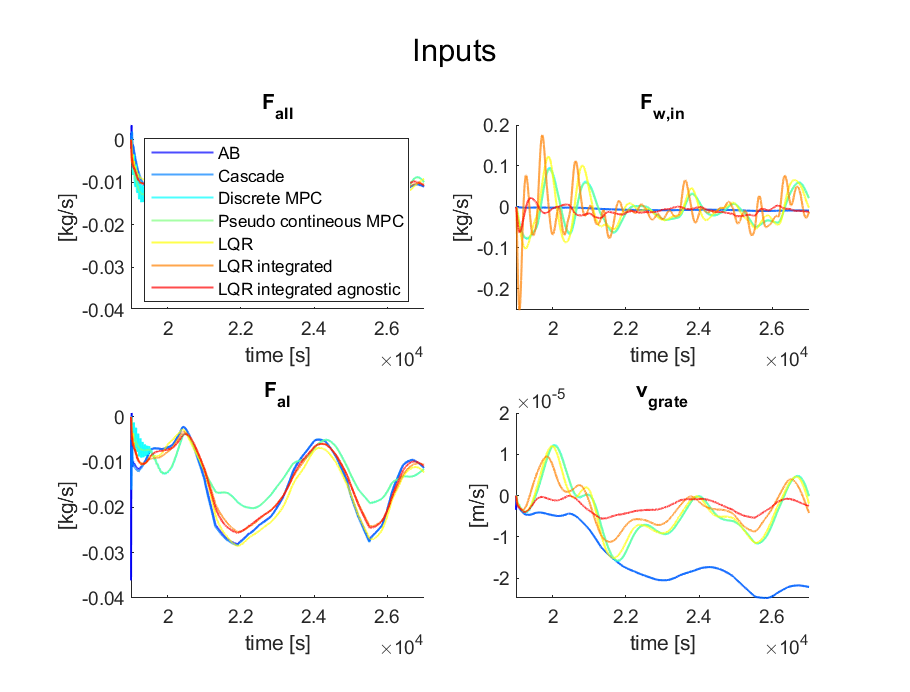
\includegraphics[width=\textwidth]{img/Fig_dump/outputs_ABCascadeDiscrete_MPCPseudo_contineous_MPCLQRLQR_integratedLQR_integrated_agnostic.eps}
    \label{fig:Assuming_controllers_outputs}
    \caption{Comparison of the different controllers with stochastic disturbances}
\end{figure}
\todo[inline]{@@@ Remove the stochastic plot}
\noindent
The solution to this would normally be a rather unpleasant one, as it involves tuning the expected disturbance for each state, and the expected noise for each input. Luckily, it is not so hard to make an estimator that functions decently, and that can stabilize the plant in combination with a gentle controller. As a result, tuning the estimator becomes part of the optimization tuning problem. 
\todo[inline]{Say something about estimators with measurements}

\subsection{Integral LQR}
Almost any model predictive controller that is not overly aggressive should be able to fulfil point 1. The second one is a bit more tricky, but the normal solution to this is to add integral states to all controlled outputs. This also has the added benefit of allowing reference tracking, even without explicitly creating a feed-forward matrix. The easiest way to get integral action for the outputs is to expand the state-space

\begin{align}
 A_{I} =& 
 \begin{bmatrix}
 A & 0 \\
 I & 0
 \end{bmatrix}\\
 B_{I} =& 
 \begin{bmatrix}
 B \\
 0
 \end{bmatrix}\\
 C_{I} =& 
 \begin{bmatrix}
 C & 0 \\
 0 & I
 \end{bmatrix}\\
  D_{I} =& 
 \begin{bmatrix}
 D \\
 0 
 \end{bmatrix}\\
\end{align}

\begin{figure}
    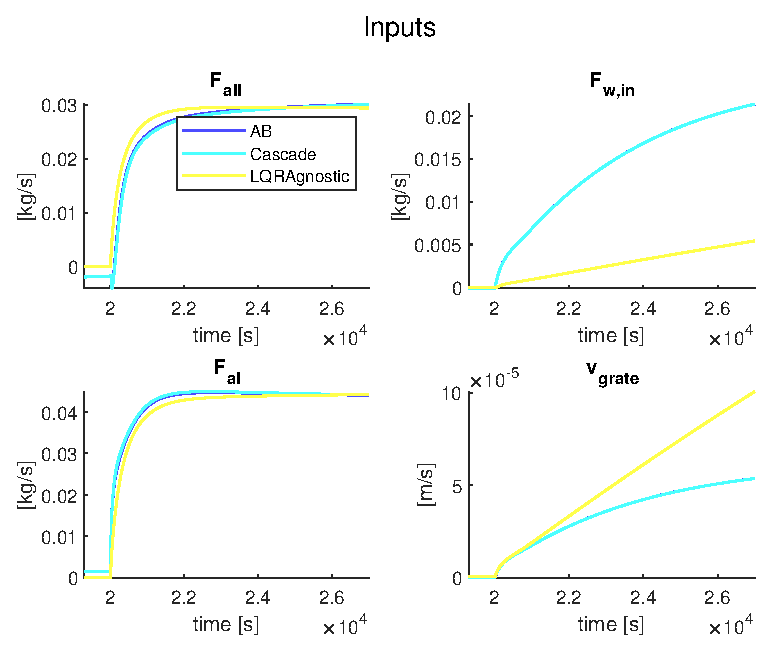
\includegraphics[width=\textwidth]{img/Fig_dump/inputs_ABCascadeLQRAgnosticStep_Q_all.eps}
    \label{fig:integral_controller_comparison}
    \caption{Normal integral cost LQR vs PID}
\end{figure}

\begin{figure}
    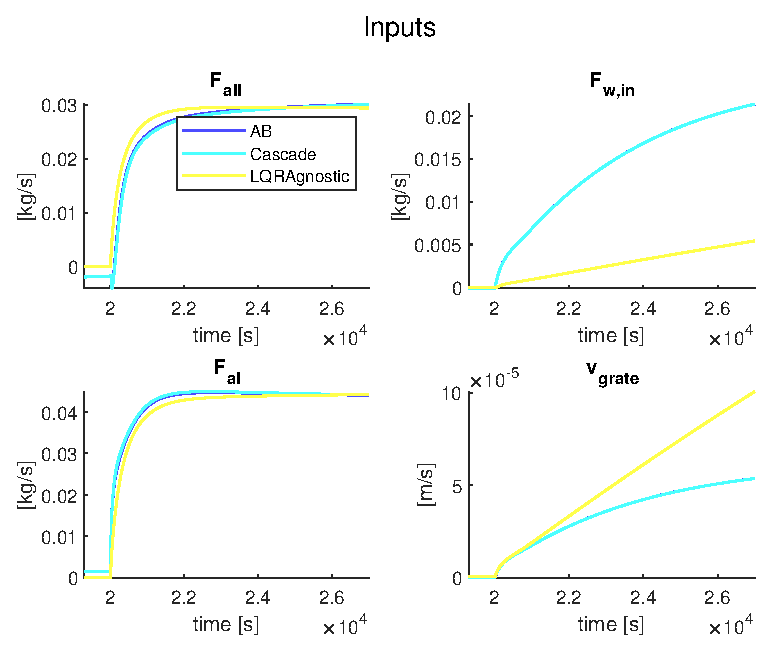
\includegraphics[width=\textwidth]{img/Fig_dump/inputs_ABCascadeLQRAgnosticStep_Q_all.eps}
    \label{fig:integral_controller_comparison_inputs}
    \caption{Normal integral cost LQR vs PID}
\end{figure}
\todo[inline]{Change the figures to how they reject noise instead}

\noindent
As can be seen in figure \ref{fig:integral_controller_comparison}, the linear quadratic controller still loses to the PID-controllers on some points. Mostly in regards to steam production and $O_2$ concentration. The reason for this is most likely some 
\todo[inline]{Should I say that it probably stems from a modeling error}

. The main draw-back is that the LQR-controller has an unintended change in the amount of air released. This also happens to the PID, but that is because the selected ratio between primary and secondary air is chosen to be different from 1.  Even if aggressive usage of primary and secondary air can be a useful tool for handling disturbances, changes in grate-speed and waste-flow should be the preferred method for handling persistent changes in waste-composition. It is possible to give an additional cost for whenever $F_{aI}$ and $F_{aII}$. The resulting controller, as seen in figure \ref{fig:integral_controller_with_air_diff_cost} loses a lot of its ability to reject disturbances properly, while also being somewhat robust.


\begin{figure}
    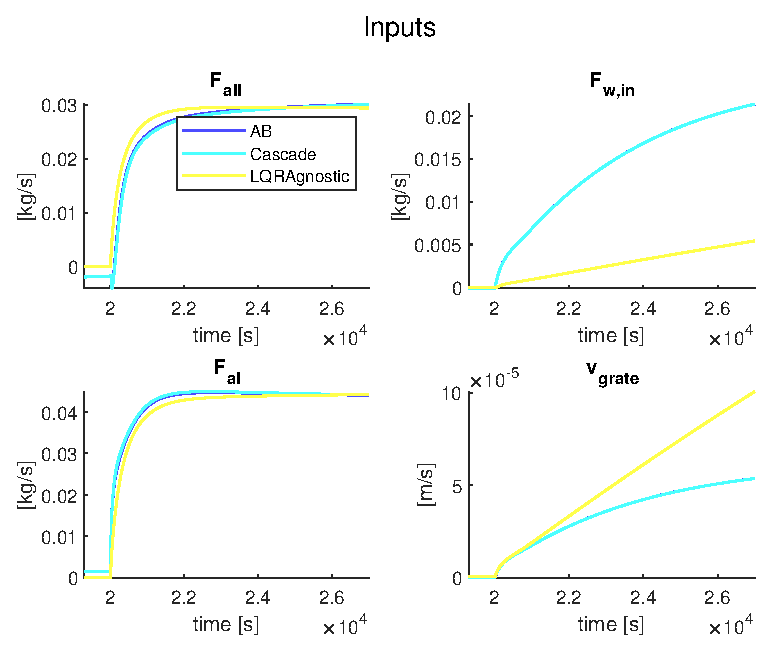
\includegraphics[width=\textwidth]{img/Fig_dump/inputs_ABCascadeLQRAgnosticStep_Q_all.eps}
    \label{fig:integral_controller_with_air_diff_cost}
    \caption{LQR versus PIDs}
\end{figure}

\begin{figure}
    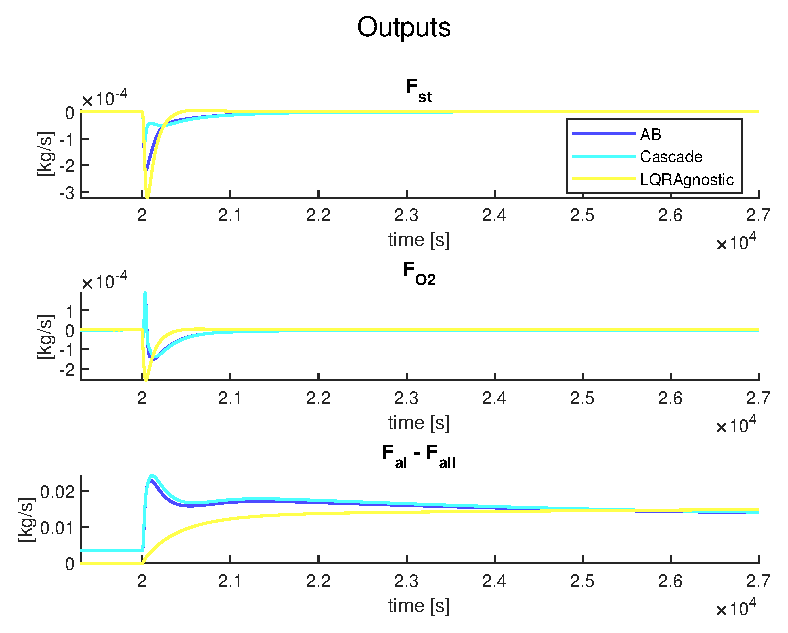
\includegraphics[width=\textwidth]{img/Fig_dump/outputs_ABCascadeLQRAgnosticStep_Q_all.eps}
    \label{fig:integral_controller_with_air_diff_cost_inputs}
    \caption{LQR versus PIDs}
\end{figure}

\todo[inline]{Say something about the differences if it can not be fixed}
\subsection{LQR with integral cost on \texorpdfstring{$F_{aI}-F_{aII}$}{TEXT}}
Balancing the normal costs, trying to reject disturbances, while also enforcing a decent ratio between $F_{aI}$ and $F_{aII}$ may prove to be a pointless endeavour. It may also mean not using a very useful tool for rejecting disturbances since allowing the two air-flows to temporarily deviate has a faster response than changing the amount of waste ted into the furnace. The intuitive solution to this is to add an integral cost to  $F_{aI}-F_{aII}$ instead, and then giving it a rather low priority compared to the other objectives. The resulting response is shown in figure \ref{fig:integrall_diff_cost_outputs}

\begin{figure}
    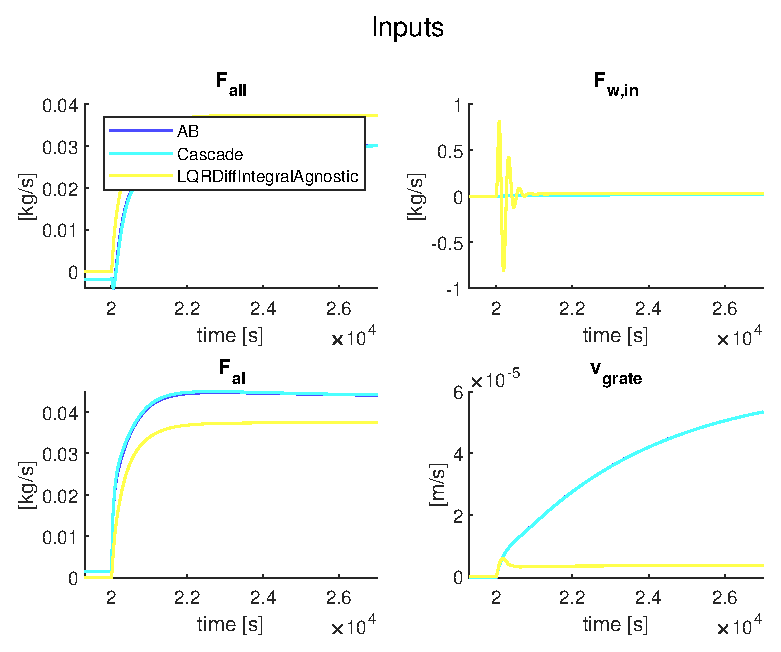
\includegraphics[width=\textwidth]{img/Fig_dump/outputs_ABCascadeLQRDiffIntegralAgnosticStep_Q_all.eps}
    \label{fig:integrall_diff_cost_outputs}
    \caption{PID vs LQR with intefral cost on $F_{aI} - F_{aII}$}
\end{figure}

\begin{figure}
    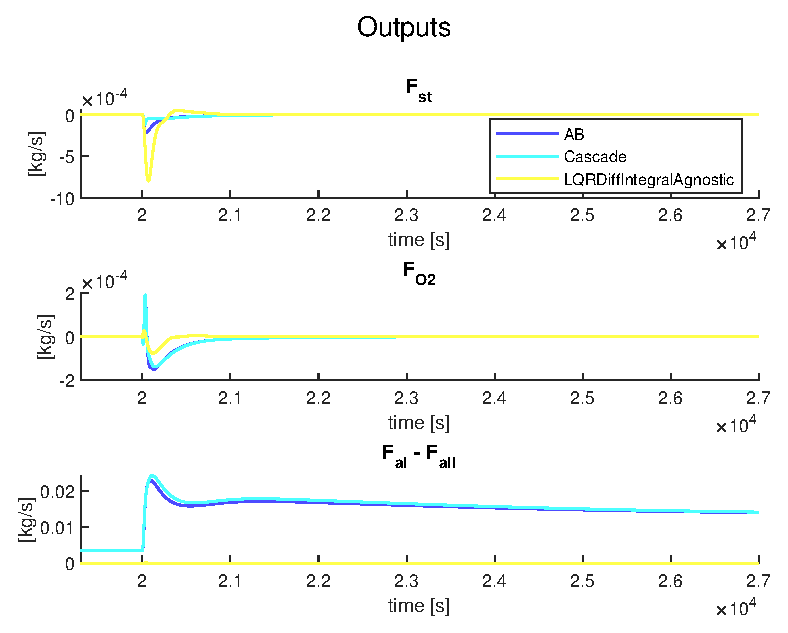
\includegraphics[width=\textwidth]{img/Fig_dump/inputs_ABCascadeLQRDiffIntegralAgnosticStep_Q_all.eps}
    \label{fig:integrall_diff_cost_inputs}
    \caption{PID vs LQR with intefral cost on $F_{aI} - F_{aII}$}
\end{figure}


\todo[inline]{C@@@ omment the results (The current ones are form an over-sensitive controller, so it might be bad...)}
% \subsection{}

\subsection{Discrete MPC}

\todo[inline]{@@@ Add an actual plot of a discrete MPC}
Even if a rather low sampling-time might work well for an MPC in practice, it does not work as well with the simulator, due to the stiffness of the problem. As a result, a sampling-time of 20 had to be chosen, even though that is noticeably slower than the preferable sampling-time of somewhere around one second. As a result, the MPC will have objectively worse performance than the LQR as long as all inequality-constraints are inactive. The delay means that the weight used for the LQR may not work as well for an MPC. The simulation will also run more slowly when an MPC is involved.
\begin{figure}
    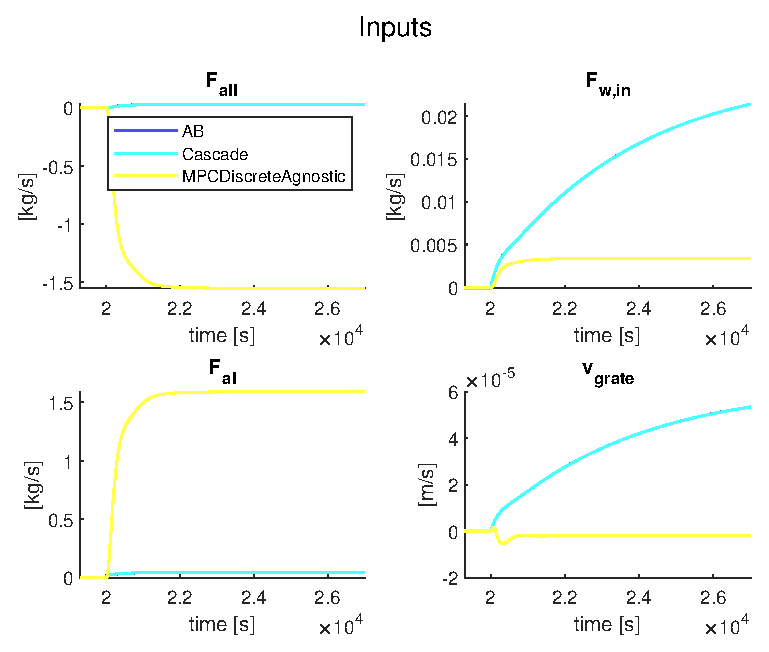
\includegraphics[width=\textwidth]{img/Fig_dump/outputs_ABCascadeMPCDiscreteAgnosticStep_Q_all.eps}
    \label{fig:discrete_mpc_outputs}
    \caption{Comparison of the different controllers with stochastic disturbances@@@}
\end{figure}

\begin{figure}
    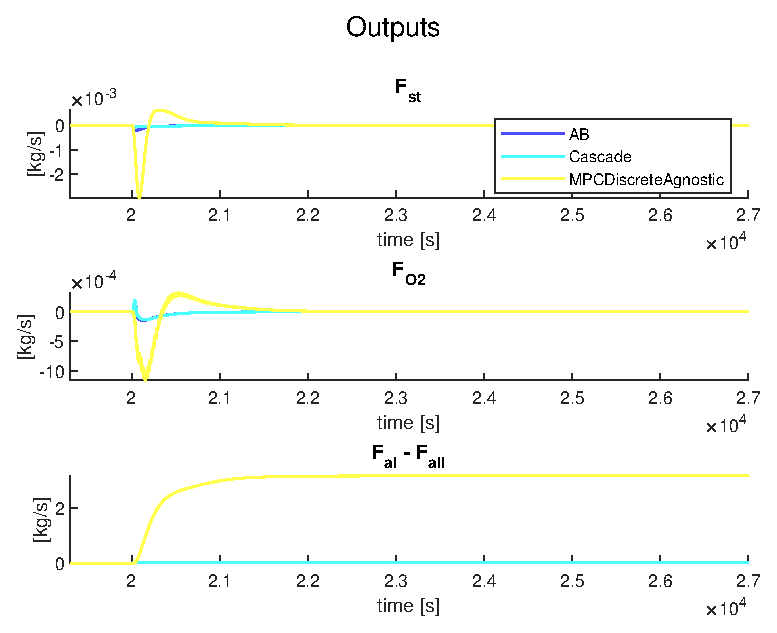
\includegraphics[width=\textwidth]{img/Fig_dump/inputs_ABCascadeMPCDiscreteAgnosticStep_Q_all.eps}
    \caption{Comparison of the different controllers with stochastic disturbances@@@}
\end{figure}


